\documentclass[conference]{IEEEtran}
\IEEEoverridecommandlockouts

\usepackage{cite}
\usepackage{amsmath,amssymb}
\usepackage{booktabs}
\usepackage{multirow}
\usepackage{array}
\usepackage{graphicx}
\usepackage{xcolor}
\usepackage{tikz}
\usetikzlibrary{positioning,arrows.meta,calc,fit,backgrounds}
\usepackage{pgfplots}
\pgfplotsset{compat=1.18}
\usepgfplotslibrary{groupplots}
\usepackage[hidelinks]{hyperref}
\usepackage{balance}

\definecolor{llm}{HTML}{F6D9B8}
\definecolor{llmline}{HTML}{B5651D}
\definecolor{det}{HTML}{FFFFFF}
\definecolor{detline}{HTML}{444444}
\definecolor{datafill}{HTML}{E4ECF5}
\definecolor{dataline}{HTML}{2F5F8F}
\definecolor{cbg}{HTML}{1F77B4}
\definecolor{cwhole}{HTML}{D62728}
\definecolor{crag}{HTML}{7F7F7F}
\definecolor{cmem}{HTML}{9467BD}

\newcommand{\st}[1]{\textsc{#1}}

\begin{document}

\title{BeliefGraph: Keeping Long-Term Agent Memory Consistent When Facts Change, with Small Open Models}

\author{\IEEEauthorblockN{Thejas Rao}
\IEEEauthorblockA{\url{https://github.com/thejasrao262003/beliefGraph}}}

\maketitle

\begin{abstract}
An assistant with long-term memory stores facts it observed and conclusions it derived from them. When a fact changes, some conclusions must be withdrawn or recomputed, some should become uncertain, and the rest should stay. Current memory systems update or invalidate the changed fact but do not track what was derived from it. Giving the model the whole store at every update works for small stores and strong models, but it breaks down on 7--12B open models as the store grows. BeliefGraph records, when a memory is written, why it is believed: a small model picks the rule that produced the memory and links the rule's conditions to stored items, giving an OR-of-AND justification. When an update arrives, the model reads only the update and its 12 nearest facts, and a truth-maintenance propagation step with no LLM assigns every memory an action. No call ever sees the whole store. Across six open models of 7--12B parameters and three datasets, BeliefGraph beats whole-store prompting and retrieval in 17 of 18 model--dataset pairs. With Gemma-4-12B it reaches a balanced accuracy of 0.935 on long dossiers, against 0.752 for whole-store prompting, 0.527 for Mem0 and 0.500 for Graphiti. On a 443-memory MQuAKE-T store it scores 0.961 using 1.4k input tokens per update; whole-store prompting uses 59k tokens and scores 0.500, the same as changing nothing. The method keeps its accuracy with 4-bit weights and a 3-bit TurboQuant KV cache on a 24\,GB laptop, where the prompting baselines lose up to 9 points. We also report the variants that did not work and where the remaining errors come from.
\end{abstract}

\begin{IEEEkeywords}
agent memory, belief revision, truth maintenance, small language models, knowledge graphs, quantization
\end{IEEEkeywords}

\section{Introduction}

An assistant that remembers across sessions accumulates two kinds of items. Some are facts it was told or observed: Priya lives in Seattle; her employer reimburses gym memberships. Others are conclusions it derived by applying a rule to those facts: it recommended a Seattle gym membership; it drafted a weekend plan that includes a Saturday gym session. When Priya moves to Austin, the gym recommendation and the plan built on it are wrong, and nothing in either memory says so. When an anonymous forum post claims the reimbursement has ended, the recommendation should stand, because it has a second, independent reason: Priya runs three times a week (Fig.~\ref{fig:example}).

This is belief revision over a store whose facts change, and it fails in two directions. A system that does not propagate leaves stale conclusions in memory. A system that withdraws every descendant of a changed fact destroys conclusions that still have support. Truth maintenance systems (TMS) solved the propagation half long ago~\cite{doyle1979,dekleer1986}. If each conclusion carries its justifications as an OR of AND-sets of premises, it survives exactly when one of its sets survives. A TMS does not say where the justifications come from. In an LLM agent nobody writes them down: a memory is a sentence, and the rule behind it was applied silently by a model at some earlier point.

Agent memory systems in use today do not record justifications. Mem0~\cite{chhikara2025mem0} decides ADD, UPDATE or DELETE for each extracted fact against similar stored items. Graphiti, the engine behind Zep~\cite{rasmussen2025zep}, invalidates contradicted edges in a temporal knowledge graph. Both can notice that ``Priya lives in Seattle'' changed. Neither knows that a gym recommendation two hops away depended on it. The other obvious approach is to give the model the whole store at every update and ask which memories to revise. That works for small stores and frontier models. It costs prompt tokens in proportion to the store, and on 7--12B open models it collapses: at 443 memories, Gemma-4-12B given the whole store does no better than changing nothing.

BeliefGraph is a justification layer that sits next to an existing memory store. When a memory is written, a small model chooses the rule that produced it and links the rule's conditions to stored facts and memories. When an update arrives, the model reads the update and its nearest facts and says which fact it changes, how (retracted, replaced or put in doubt), and how reliable the source is. A deterministic propagation over the graph then decides an action for every memory: keep, withdraw, recompute or mark uncertain. Every call is narrow, so a 12B model is enough, and the cost of an update does not grow with the store.

Our contributions are:
\begin{enumerate}
\item A decomposition of justification induction into small, constrained calls that 7--12B models handle without fine-tuning: rule routing from token probabilities with a joint per-entity assignment, and sampled grounding (Section~\ref{sec:method}). We also describe the variants we tried on the way, including five that did not help (Section~\ref{sec:tried}).
\item An evaluation with gold revision labels on four datasets: a new long-dossier set and conversions of ProofWriter, STALE and MQuAKE-T. We compare against whole-store prompting, retrieval, Mem0 and Graphiti, across six open models (Section~\ref{sec:results}).
\item An attribution of the remaining errors to graph building or update reading, made by swapping in gold components over cached calls.
\item A deployment study covering FP8, INT4 and 2--8-bit GGUF weights, quantized KV caches including TurboQuant~\cite{zandieh2026turboquant}, and an end-to-end run on a laptop.
\end{enumerate}

\begin{figure}[t]
\centering
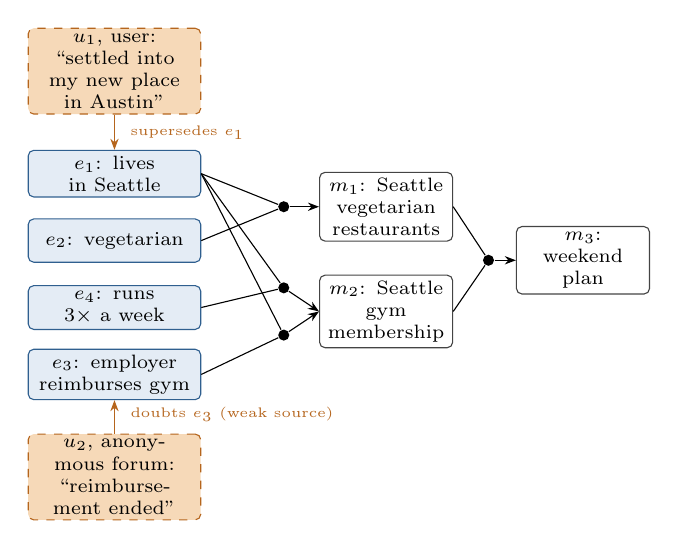
\begin{tikzpicture}[
  font=\scriptsize,
  ev/.style={draw=dataline, fill=datafill, rounded corners=2pt, text width=2.05cm, align=center, inner sep=2pt, minimum height=0.55cm},
  mem/.style={draw=detline, fill=white, rounded corners=2pt, text width=1.55cm, align=center, inner sep=2pt, minimum height=0.55cm},
  up/.style={draw=llmline, fill=llm, dashed, rounded corners=2pt, text width=2.05cm, align=center, inner sep=2pt},
  j/.style={circle, fill=black, inner sep=0pt, minimum size=4pt},
  a/.style={-{Stealth[length=4pt]}, thin},
  l/.style={thin}
]
\node[ev] (e1) at (0,3.0) {$e_1$: lives in Seattle};
\node[ev] (e2) at (0,2.15) {$e_2$: vegetarian};
\node[ev] (e4) at (0,1.3) {$e_4$: runs 3$\times$ a week};
\node[ev] (e3) at (0,0.45) {$e_3$: employer reimburses gym};
\node[up, anchor=south] (u1) at (0,3.75) {$u_1$, user: ``settled into my new place in Austin''};
\node[up, anchor=north] (u2) at (0,-0.3) {$u_2$, anonymous forum: ``reimbursement ended''};
\draw[a, llmline] (u1) -- (e1);
\draw[a, llmline] (u2) -- (e3);
\node[font=\tiny, text=llmline, anchor=west] at (0.08,3.52) {supersedes $e_1$};
\node[font=\tiny, text=llmline, anchor=west] at (0.08,-0.06) {doubts $e_3$ (weak source)};

\node[j] (j1) at (2.15,2.58) {};
\node[j] (j2) at (2.15,1.55) {};
\node[j] (j3) at (2.15,0.95) {};
\node[mem] (m1) at (3.45,2.58) {$m_1$: Seattle vegetarian restaurants};
\node[mem] (m2) at (3.45,1.25) {$m_2$: Seattle gym membership};
\node[j] (j4) at (4.75,1.9) {};
\node[mem] (m3) at (5.95,1.9) {$m_3$: weekend plan};

\draw[l] (e1.east) -- (j1); \draw[l] (e2.east) -- (j1);
\draw[l] (e1.east) -- (j2); \draw[l] (e4.east) -- (j2);
\draw[l] (e1.east) -- (j3); \draw[l] (e3.east) -- (j3);
\draw[a] (j1) -- (m1); \draw[a] (j2) -- (m2.west); \draw[a] (j3) -- (m2.west);
\draw[l] (m1.east) -- (j4); \draw[l] (m2.east) -- (j4);
\draw[a] (j4) -- (m3);
\end{tikzpicture}
\caption{A memory store with its justification graph. Each black dot is one justification: an AND of its inputs. A memory with two dots ($m_2$, under the rule ``recommend a local gym if the user exercises regularly \emph{or} the employer pays'') holds if either dot holds. After $u_1$, $m_1$, $m_2$ and $m_3$ must all be recomputed. After $u_2$ alone, $e_3$ becomes uncertain, but $m_2$ is kept through $\{e_1,e_4\}$.}
\label{fig:example}
\end{figure}

\section{Related Work}

\textit{Truth maintenance and belief revision.} A justification-based TMS labels a node IN if any of its justifications is valid~\cite{doyle1979}. The assumption-based TMS computes, for each datum, the assumption sets it holds under, from justifications that the problem solver supplies~\cite{dekleer1986}. de Kleer already named the over-retraction problem: only assertions directly affected by a contradiction should be retracted, and it is costly to find out which ones those are. The AGM postulates~\cite{agm1985} describe rational revision of logically closed theories. Veritas-TMS~\cite{veritas} packages an OR-of-AND JTMS for agent memory, with justifications passed in by the caller. Our propagation step is a JTMS-style labeller with two extra states (uncertain and stale), and we do not claim it as new. What we study is how to obtain the justifications from text with small models, and how much accuracy that costs.

\textit{Agent memory.} MemGPT~\cite{packer2023memgpt}, Mem0~\cite{chhikara2025mem0} and Zep/Graphiti~\cite{rasmussen2025zep} store and retrieve memories; Mem0 and Graphiti also update or invalidate stored facts. Kumiho~\cite{park2026kumiho} gives graph-native memory formal belief-revision semantics and includes LLM-driven edge discovery, but it does not measure edge accuracy or downstream revision. NeuSymMS~\cite{sultan2026neusymms} and Belief Memory~\cite{liao2026beliefmemory} add symbolic and probabilistic structure. The closest work is PACMI~\cite{wang2026pacmi}, which cascades invalidation along annotated provenance edges on two-hop chains. Its appendix proposes branching topologies and text-induced edges as future work. Invalidation Contracts~\cite{wu2026invalidation} evict cached results using dependency vectors that the server declares. StateAuditor~\cite{sun2026stateauditor} repairs responses that depend on stale state. Goswami et al.~\cite{goswami2026rederive} find that agents retrieve updated premises but keep following old conclusions. As far as we can tell, none of these induces AND/OR structure from text or measures over-invalidation of conclusions that still have support.

\textit{Benchmarks.} STALE~\cite{chao2026stale} asks whether agents notice that a memory is no longer valid, including conflicts that reach it indirectly. BeliefShift~\cite{myakala2026beliefshift}, AGM-Bench~\cite{jenkins2026agmbench} and DeltaLogic~\cite{dhanda2026deltalogic} test revision in context, with every premise in the prompt; DeltaLogic's over-flip rate is the in-context counterpart of our over-invalidation rate. MQuAKE~\cite{zhong2023mquake} and RippleEdits~\cite{cohen2024ripple} test the multi-hop consequences of edits to a model's parametric knowledge. We reuse MQuAKE-T's real Wikidata edits as a stored-memory task, and convert ProofWriter~\cite{tafjord2021proofwriter} proofs into gold justification graphs.

\textit{Quantization.} TurboQuant~\cite{zandieh2026turboquant} quantizes vectors online: a random rotation makes every coordinate follow a known distribution, which is then quantized with a Lloyd--Max codebook~\cite{lloyd1982,max1960}. Its main target is the KV cache. We use it to test whether BeliefGraph's short calls tolerate aggressive cache compression.

\section{Problem Setting}
\label{sec:problem}

A store holds facts $E$, rules $P$ and memories $M$, all as text. Each fact $e$ has a source, an observation time $t(e)$ and a source reliability $r(e)\in\{\text{low},\text{medium},\text{high}\}$. Each memory $m$ was produced by one rule from premises in $E\cup M$. Its justification is a set of alternatives $J(m)=\{A_1,\dots,A_k\}$, each $A_i\subseteq E\cup M$ a conjunction. The graph is acyclic.

Updates arrive one at a time as text with a source and a time. The gold reading of an update $u$ is a target fact $e$, a relation $\rho\in\{\text{retracts},\text{supersedes},\text{hedges}\}$ and a reliability $r(u)$. Some updates are implicit and do not mention the fact they change.

Statuses are ordered $\st{out}<\st{unk}<\st{stale}<\st{in}$. An update sets the status of its target to
\begin{equation}
\sigma(e)=\begin{cases}
\st{in} & t(u)<t(e)\ \text{(outdated update)}\\
\st{unk} & \rho=\text{hedges or } r(u)<r(e)\\
\st{out} & \rho=\text{retracts}\\
\st{stale} & \rho=\text{supersedes,}
\end{cases}
\end{equation}
taking the minimum when several updates hit one fact. Untouched facts are \st{in}. Memories follow in topological order:
\begin{equation}
\sigma(m)=\max_{A\in J(m)}\ \min_{x\in A}\ \sigma(x).
\label{eq:prop}
\end{equation}
The action for a memory is keep (\st{in}), recompute (\st{stale}), uncertain (\st{unk}) or withdraw (\st{out}). Gold actions come from (\ref{eq:prop}) over gold justifications and gold readings.

\textit{Metrics.} A memory is \emph{revising} if its gold action is not keep. The stale rate is the share of revising memories a system keeps. The over-invalidation rate is the share of gold-keep memories it changes. Balanced accuracy is $1-(\text{stale}+\text{over-invalidation})/2$, computed per store after the last update and averaged over stores. Changing nothing scores 0.5, and so does changing everything. Most memories in a large store should be kept, so plain accuracy rewards inaction; we report it only for the first, small-store study, where it means exact action match.

\section{BeliefGraph}
\label{sec:method}

\begin{figure*}[t]
\centering
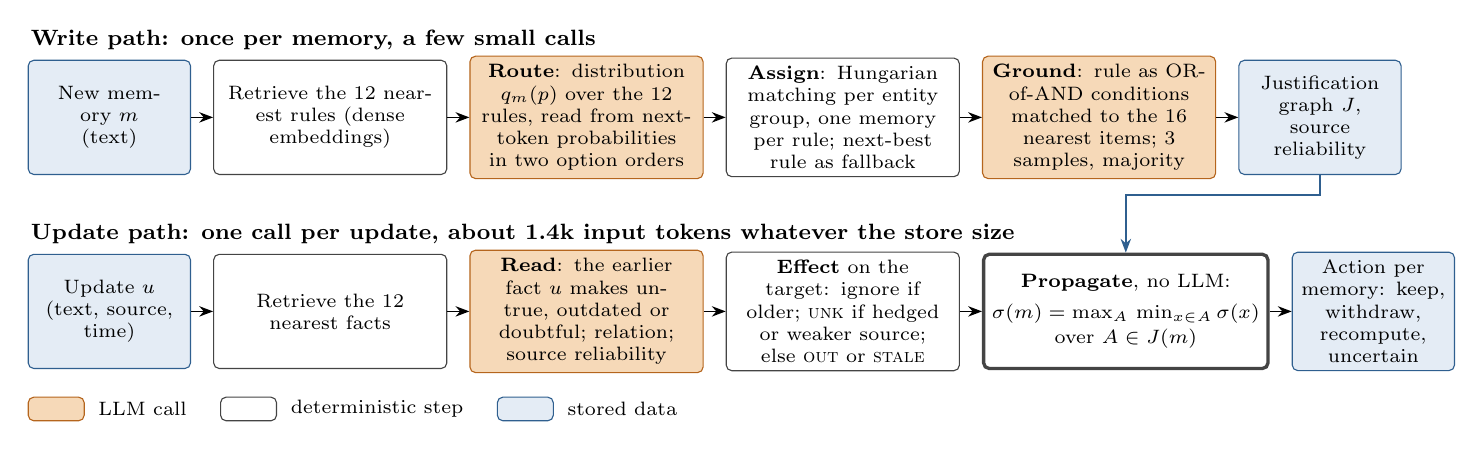
\begin{tikzpicture}[
  font=\scriptsize,
  box/.style={draw=detline, fill=det, rounded corners=2pt, text width=2.75cm, align=center, inner sep=3pt, minimum height=1.45cm},
  llmbox/.style={box, draw=llmline, fill=llm},
  data/.style={box, draw=dataline, fill=datafill, text width=1.85cm},
  a/.style={-{Stealth[length=5pt]}, semithick},
  lane/.style={font=\footnotesize\bfseries, anchor=south west, inner sep=1pt}
]
% write path
\node[data] (a0) at (0,0) {New memory $m$\\(text)};
\node[box, right=0.28cm of a0] (a1) {Retrieve the 12 nearest rules (dense embeddings)};
\node[llmbox, right=0.28cm of a1] (a2) {\textbf{Route}: distribution $q_m(p)$ over the 12 rules, read from next-token probabilities in two option orders};
\node[box, right=0.28cm of a2] (a3) {\textbf{Assign}: Hungarian matching per entity group, one memory per rule; next-best rule as fallback};
\node[llmbox, right=0.28cm of a3] (a4) {\textbf{Ground}: rule as OR-of-AND conditions matched to the 16 nearest items; 3 samples, majority};
\node[data, right=0.28cm of a4] (a5) {Justification graph $J$, source reliability};
\draw[a] (a0) -- (a1); \draw[a] (a1) -- (a2); \draw[a] (a2) -- (a3); \draw[a] (a3) -- (a4); \draw[a] (a4) -- (a5);
\node[lane] at ($(a0.north west)+(0,0.08)$) {Write path: once per memory, a few small calls};
% update path
\node[data, below=1.0cm of a0] (b0) {Update $u$\\(text, source, time)};
\node[box, right=0.28cm of b0] (b1) {Retrieve the 12 nearest facts};
\node[llmbox, right=0.28cm of b1] (b2) {\textbf{Read}: the earlier fact $u$ makes untrue, outdated or doubtful; relation; source reliability};
\node[box, right=0.28cm of b2] (b3) {\textbf{Effect} on the target: ignore if older; \st{unk} if hedged or weaker source; else \st{out} or \st{stale}};
\node[box, right=0.28cm of b3, very thick, text width=3.4cm] (b4) {\textbf{Propagate}, no LLM:\\[3pt] ${\sigma(m)=\max_{A}\,\min_{x\in A}\sigma(x)}$\\[1pt] over ${A\in J(m)}$};
\node[data, right=0.28cm of b4] (b5) {Action per memory: keep, withdraw, recompute, uncertain};
\draw[a] (b0) -- (b1); \draw[a] (b1) -- (b2); \draw[a] (b2) -- (b3); \draw[a] (b3) -- (b4); \draw[a] (b4) -- (b5);
\node[lane] at ($(b0.north west)+(0,0.08)$) {Update path: one call per update, about 1.4k input tokens whatever the store size};
\draw[a, dataline] (a5.south) -- ++(0,-0.25) -| (b4.north);
% legend
\node[llmbox, minimum height=0.3cm, text width=0.5cm, below=0.35cm of b0.south west, anchor=north west] (l1) {};
\node[right=0.05cm of l1, font=\scriptsize] (l1t) {LLM call};
\node[box, minimum height=0.3cm, text width=0.5cm, right=0.3cm of l1t] (l2) {};
\node[right=0.05cm of l2, font=\scriptsize] (l2t) {deterministic step};
\node[data, minimum height=0.3cm, text width=0.5cm, right=0.3cm of l2t] (l3) {};
\node[right=0.05cm of l3, font=\scriptsize] {stored data};
\end{tikzpicture}
\caption{BeliefGraph v0.8. The write path runs once per memory and records why the memory is believed. The update path runs once per update and reads only the update and its nearest facts. Revision is a deterministic propagation over the recorded graph.}
\label{fig:arch}
\end{figure*}

Fig.~\ref{fig:arch} shows the system. It wraps any chat model behind an OpenAI-compatible or vendor API. All candidate lists come from dense retrieval with nomic-embed-text-v1.5~\cite{nussbaum2024nomic}.

\textit{Source reliability.} Source descriptions (``HR benefits email'', ``anonymous forum post'') are rated high, medium or low in batches of 40.

\textit{Routing.} For a new memory $m$ we take the 12 rules nearest to it and show them as lettered options. Instead of generating an answer, we prefill the assistant turn up to the option letter and read the next-token probabilities over the letters. We do this for the original and the reversed option order and average, which gives a distribution $q_m$ over the 12 candidates. Each pass is a single forward step.

\textit{Joint assignment.} Memories that name the same entity form a group. Within a group, a rule produces at most one memory: the gym rule yields one gym recommendation for Priya, not two. We solve $\max\sum_m \log q_m(p_m)$ under that constraint with the Hungarian algorithm~\cite{kuhn1955}. This targets the most common routing error we saw: a downstream memory sent to the rule that grants its premise instead of the rule that grants the memory itself. Both rules look relevant to the memory on their own. Only the group view shows that the premise's rule is already taken by another memory. If the assigned rule cannot be grounded, the next-best rule is tried, at most twice.

\textit{Grounding.} Given the rule and the memory, the model rewrites the rule's condition as OR-of-AND conditions and matches each condition to one of the 16 facts or memories nearest to the memory, by id. We draw three seeded samples and keep a justification set if most samples produce it, else the most frequent complete set. Cycles are broken by dropping the fewest edges. A memory left with no justification gets one more call on its own. If it is still unsupported, it is reported to the caller rather than silently kept.

\textit{Update reading.} Each update gets one call with the update and the 12 facts nearest to it. The prompt asks for the earlier fact that the update makes untrue, outdated or doubtful, including by implication, plus the relation and the source's reliability. The relation is decided by what the update asserts, not by who asserts it. A weak source flatly denying a fact is still a retraction; Eq.~(1) turns it into doubt because the source is weaker than the original.

\textit{Revision.} Eq.~(\ref{eq:prop}) runs over the induced graph and the readings. It takes milliseconds and makes no model call. Memories marked recompute are handed back to the caller; we do not generate or score the recomputed text in this paper.

\textit{Cost.} Building costs about 4--5k input tokens per memory, once. An update costs one call of 0.8--1.4k input tokens, independent of the store size. Whole-store prompting pays for the entire store at every update.

\section{What We Tried}
\label{sec:tried}

\begin{table}[t]
\caption{Variants in the order we built them. Scores are balanced accuracy unless marked; ``touched'' is plain accuracy on memories of scenarios that received an update.}
\label{tab:versions}
\centering
\footnotesize
\setlength{\tabcolsep}{3pt}
\begin{tabular}{@{}>{\raggedright\arraybackslash}p{0.95cm}>{\raggedright\arraybackslash}p{3.65cm}>{\raggedright\arraybackslash}p{2.9cm}@{}}
\toprule
Version & Change & Effect \\
\midrule
v0 & One call builds the whole graph; one call reads all updates & Opus 0.990 accuracy, small stores \\
v0.1 & Retry and report unsupported memories & Basis for Table~\ref{tab:small} \\
v0.2 & Per memory: route among 12 rules, ground on 16 items; read each update on 5 facts & Qwen-9B, 143 mem.: touched 0.749$\to$0.864 \\
read-v2 & Relation from the assertion, not the source & 0.864$\to$0.932 touched \\
v0.3 & Route on a gives/requires summary of each rule & First pick 41$\to$35 of 45; \textbf{off} \\
v0.4 & 3 seeded samples, vote; adjudicate split votes & 0.932$\to$0.947 touched \\
v0.5 & Yes/no routing and name-filtered grounding for sub-4B models & Worse for 9B/4B; \textbf{off} \\
v0.6 & One rule per entity: losers re-routed & Qwen-9B dossiers 0.751$\to$0.797 \\
v0.7 & Route on the rule's THEN clause & Gemma dossiers 0.846$\to$0.824; \textbf{off} \\
v0.8 & Probability routing + Hungarian assignment & Gemma dossiers 0.846$\to$0.935 \\
reader v3 & Implicit updates, 12 candidate facts & STALE (v1 stores) 0.658$\to$0.788 \\
\midrule
\multicolumn{3}{@{}>{\raggedright\arraybackslash}p{7.95cm}@{}}{\textbf{Also off:} overlap-conflict re-routing (fired once in 93 memories, changed nothing); a 4B reranker (ranked the right rule first less often than Gemma's own choice); 0--10 relevance scores; a confidence gate on the assignment.}\\
\bottomrule
\end{tabular}
\end{table}

Table~\ref{tab:versions} lists every variant we built. Three lessons came out of this sequence.

\textit{One call per graph does not scale.} v0 asked the model to write the whole justification graph in one call. Claude Opus 5.5 did this almost perfectly on stores of 3--12 memories (justification-set F1 0.994). On merged stores of 143 memories, Qwen3.5-9B with one call per batch of 25 memories reached 0.749 touched accuracy, about the same as giving it the whole store. Splitting the work into one routing and one grounding decision per memory, each over a short candidate list, was the largest single gain.

\textit{Routing errors are systematic, so voting has a ceiling.} Sampling each decision three times and sending split votes to an adjudication call raised the right graphs from 73 to 78 of 93 memories on a hard subset. Vote share turned out to be calibrated: split votes were wrong 8 times in 13, unanimous ones 8 times in 80. But for most of the remaining wrong routes, the right rule got no vote at all, which matches what self-consistency~\cite{wang2023selfconsistency} and sample-vote-constrain pipelines such as AbsCon~\cite{chen2025abscon} would predict. Diagnosis on the long dossiers showed why: every wrong rule was another memory's rule, because all memories in a dossier concern the same person or product. That pointed to a constraint across memories (v0.6, then v0.8) rather than more samples. Moving from votes to token probabilities let the Hungarian step trade off confidences across a whole group. On 36 dossiers it raised the share of correctly assigned rules from 0.791 to 0.941.

\textit{Rewording the input rarely helped.} Summarising rules (v0.3), routing on their THEN clause (v0.7) and adding a reranker all lost information that the router had been using. The changes that worked kept the model's decisions small and added structure around them.

Thinking mode was a practical trap. In the early large-store runs, Qwen3.5-9B with thinking on spent the whole 16k output budget reasoning about whole-store prompts and returned an empty answer at 40 of 43 steps on the 143-memory store. Our parser treats an empty answer as ``keep everything''. We report those runs as they are, and ran Qwen with thinking off in the later ladder.

\section{Experimental Setup}
\label{sec:setup}

\begin{table}[t]
\caption{Datasets. Every store comes with gold justifications and gold update readings; gold actions follow from Eq.~(\ref{eq:prop}).}
\label{tab:data}
\centering
\footnotesize
\setlength{\tabcolsep}{2.5pt}
\begin{tabular}{@{}llrrr@{}}
\toprule
Dataset & Source & Stores & Memories & Updates \\
\midrule
Small scenarios & ours & 63 & 301 & 1--4 each \\
Merged streams & ours & 3 & 45 / 143 / 301 & 12 / 43 / 84 \\
Long dossiers & ours & 36 & 579 & 209 \\
ProofWriter & \cite{tafjord2021proofwriter} & 36 & 266 & 159 \\
STALE v2 & \cite{chao2026stale} & 37 & 296 & 185 \\
MQuAKE-T & \cite{zhong2023mquake} & 36 / 1 / 1 & 423 / 140 / 443 & 70 / 96 / 96 \\
\bottomrule
\end{tabular}
\end{table}

\textit{Datasets} (Table~\ref{tab:data}). Our own data starts from a graph: a generator samples a justification structure, a deterministic labeller computes gold actions, and only then is each node rendered to text by Gemini 3.5 Flash. Rendered scenarios pass automatic leak and consistency checks (no memory may state its own justification) and a review. We differentially tested the labeller against Veritas-TMS. The 63 small scenarios cover chains, multiple OR supports, AND premises with an alternative, and weak or hedged updates. Long dossiers compose 4--7 such motifs around one entity with shared facts and 4--8 updates, so many memories look alike. ProofWriter~\cite{tafjord2021proofwriter} (depth 5, natural-language rules, open-world without negation) gives its gold graph through the proofs; we add updates. STALE~\cite{chao2026stale} gives plans that rest on old statements, with implicit updates; we pack stores so that no update has two plausible targets. MQuAKE-T~\cite{zhong2023mquake} gives real Wikidata edits with multi-hop consequences; we deduplicate facts and rules within each store.

\textit{Models.} The open models are Gemma-4-12B-it (our baseline), Qwen3.5-9B, Granite-4.1-8B, Llama-3.1-8B, Ministral-3-8B and Olmo-3-7B, plus Qwen3.5-4B/2B/0.8B and Phi-4-mini for a size ladder. All are served unmodified with vLLM~\cite{kwon2023vllm} on single NVIDIA H100 or L40S GPUs; none is fine-tuned. Claude Opus 5.5 and Haiku 5.5 appear only in the first study. Every call is cached, so every reported run replays without model access.

\textit{Baselines.} All baselines use the same model, stores, updates and gold. \emph{Whole store}: the model sees every fact, rule and memory plus the updates so far, with the same label definitions, and returns an action per memory. \emph{RAG}~\cite{lewis2020rag}: the same prompt restricted to the 8 items and 4 rules nearest to each update. \emph{Mem0} 1.0.5: facts, memories and rules are stored as existing Mem0 memories; each update arrives as a user message; DELETE maps to withdraw and UPDATE to recompute. \emph{Graphiti} 0.31.2 (FalkorDB Lite backend): everything is ingested as episodes; a memory is withdrawn once any edge extracted from it is invalidated. Mem0 and Graphiti share BeliefGraph's model server and embedder. Two rule-based floors use the gold graph: \emph{direct only} revises the named fact and nothing else; \emph{naive cascade} withdraws every descendant.

\section{Results}
\label{sec:results}

\subsection{Small stores: the gain grows as the model gets weaker}

\begin{table}[t]
\caption{63 small scenarios, 301 memories, all updates at once. Exact-action accuracy; paired difference with scenario-bootstrap 95\% CI and exact McNemar test.}
\label{tab:small}
\centering
\footnotesize
\setlength{\tabcolsep}{3pt}
\begin{tabular}{@{}lccll@{}}
\toprule
Model & BG & Whole & Difference [95\% CI] & $p$ \\
\midrule
Opus 5.5 & 0.993 & 0.993 & \phantom{+}0.000 & 1.0 \\
Haiku 5.5 & 0.980 & 0.917 & +0.063 [0.013, 0.120] & $3\!\times\!10^{-4}$ \\
Qwen3.5-9B & 0.970 & 0.834 & +0.136 [0.067, 0.210] & $1\!\times\!10^{-8}$ \\
\midrule
\multicolumn{5}{@{}l}{Gold graph, no LLM: direct only 0.674; naive cascade 0.528} \\
\bottomrule
\end{tabular}
\end{table}

Table~\ref{tab:small} is where we started, and it was humbling. On small stores a frontier model gets nothing from the graph: Opus makes the same predictions with and without it. The two rule-based floors show that the task is not trivial. Naive cascade over-invalidates 37\% of memories that should stay, and direct-only leaves every derived conclusion stale. The picture changes as the model gets weaker. Haiku given the whole store leaves 11\% of revising memories stale against 2\% with BeliefGraph, and recalls only 63\% of the uncertain cases against 95\%. Its largest losses come where every alternative support has to be checked before a conclusion can go. Qwen3.5-9B builds noticeably imperfect graphs (justification-set F1 0.82), yet propagation over them beats its direct judgement in every scenario family. With the gold graph, Qwen reaches 0.993.

\subsection{Six open models, three datasets}

\begin{table*}[t]
\caption{Balanced accuracy of BeliefGraph v0.8 (BG), whole-store prompting (Whole) and retrieval (RAG), same model in each row. Best in each group in bold.}
\label{tab:ladder}
\centering
\footnotesize
\begin{tabular}{@{}lccc@{\hspace{14pt}}ccc@{\hspace{14pt}}ccc@{}}
\toprule
& \multicolumn{3}{c}{Long dossiers (579 mem.)} & \multicolumn{3}{c}{ProofWriter (266 mem.)} & \multicolumn{3}{c}{STALE v2 (296 mem.)} \\
\cmidrule(r{14pt}){2-4}\cmidrule(r{14pt}){5-7}\cmidrule{8-10}
Model & BG & Whole & RAG & BG & Whole & RAG & BG & Whole & RAG \\
\midrule
Gemma-4-12B & \textbf{0.935} & 0.752 & 0.730 & \textbf{0.847} & 0.620 & 0.636 & \textbf{0.892} & 0.756 & 0.750 \\
Qwen3.5-9B & \textbf{0.841} & 0.595 & 0.641 & \textbf{0.901} & 0.531 & 0.490 & \textbf{0.787} & 0.599 & 0.689 \\
Granite-4.1-8B & \textbf{0.831} & 0.633 & 0.654 & \textbf{0.856} & 0.664 & 0.635 & \textbf{0.777} & 0.706 & 0.664 \\
Ministral-3-8B & \textbf{0.854} & 0.625 & 0.607 & \textbf{0.836} & 0.514 & 0.569 & \textbf{0.841} & 0.594 & 0.663 \\
Llama-3.1-8B & \textbf{0.779} & 0.540 & 0.653 & \textbf{0.759} & 0.401 & 0.594 & \textbf{0.685} & 0.492 & 0.667 \\
Olmo-3-7B & \textbf{0.696} & 0.537 & 0.618 & \textbf{0.618} & 0.456 & 0.544 & 0.512 & 0.531 & \textbf{0.653} \\
\bottomrule
\end{tabular}
\end{table*}

Table~\ref{tab:ladder} runs v0.8 on six open models. BeliefGraph wins 17 of the 18 model--dataset pairs, typically by 15--30 points. The exception is Olmo-3-7B on STALE, where updates never name their target. Olmo finds the right earlier statement for only 62 of 185 updates (Gemma: 154), and its graph cannot compensate. On merged streams the whole-store baseline mostly gives up. On the 143-memory stream with thinking off, every model's whole-store answers score between 0.495 and 0.529. Most models keep everything; Llama flags 98\% of memories that should stay. BeliefGraph v0.4 scores 0.678--0.921 on the same stream.

\subsection{Memory systems}

\begin{table}[t]
\caption{Memory systems with Gemma-4-12B. Balanced accuracy.}
\label{tab:memsys}
\centering
\footnotesize
\setlength{\tabcolsep}{3pt}
\begin{tabular}{@{}lccccc@{}}
\toprule
Dataset & BG & Whole & RAG & Mem0 & Graphiti \\
\midrule
Long dossiers & \textbf{0.935} & 0.752 & 0.730 & 0.527 & 0.500 \\
ProofWriter & \textbf{0.847} & 0.620 & 0.636 & 0.500 & 0.489 \\
STALE v2 & \textbf{0.892} & 0.756 & 0.750 & 0.684 & 0.500 \\
MQuAKE-T, $\sim$12 mem. & 0.963 & \textbf{0.984} & 0.725 & 0.594 & -- \\
MQuAKE-T, 140 mem. & \textbf{0.988} & 0.717 & 0.642 & 0.533 & 0.538 \\
MQuAKE-T, 443 mem. & \textbf{0.961} & 0.500 & 0.646 & 0.532 & -- \\
\bottomrule
\end{tabular}
\end{table}

Mem0 and Graphiti were not designed for this task, and Table~\ref{tab:memsys} shows it. Mem0 does notice change: it updates or deletes the fact an update targets for 39--75\% of updates. But on the dossiers, ProofWriter and the large MQuAKE stores, only 1--15\% of updates lead it to touch any stored conclusion. It does better on STALE and the small MQuAKE stores (38--47\%), where a plan rests on a single fact and is often worded like it, so similarity search finds it. Graphiti invalidates contradicted edges but never touches a derived conclusion, and stays at or near 0.5 everywhere. Both systems would need a notion of ``derived from'' to do better. Adding one is the contribution of this paper.

\subsection{Cost and scale}

\begin{figure}[t]
\centering
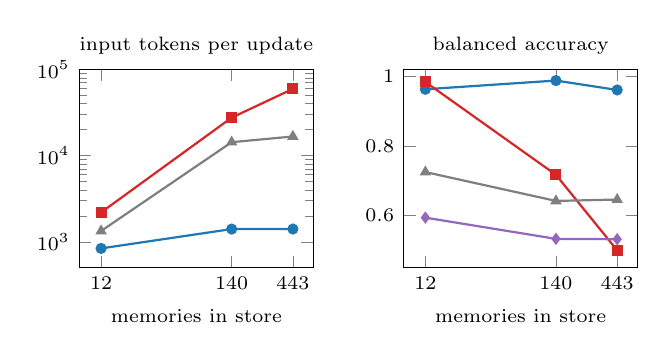
\begin{tikzpicture}
\begin{groupplot}[
  group style={group size=2 by 1, horizontal sep=1.15cm},
  width=4.55cm, height=4.1cm,
  xmode=log, xmin=8, xmax=650,
  xtick={12,140,443}, xticklabels={12,140,443},
  xlabel={memories in store},
  tick label style={font=\scriptsize}, label style={font=\scriptsize},
  title style={font=\scriptsize, yshift=-4pt},
  every axis plot/.append style={thick, mark size=1.6pt},
]
\nextgroupplot[ymode=log, ymin=500, ymax=100000, title={input tokens per update},
  ytick={1000,10000,100000}]
\addplot[cbg, mark=*] coordinates {(12,838) (140,1405) (443,1406)};
\addplot[cwhole, mark=square*] coordinates {(12,2192) (140,27586) (443,59486)};
\addplot[crag, mark=triangle*] coordinates {(12,1334) (140,14318) (443,16666)};
\nextgroupplot[ymin=0.45, ymax=1.02, title={balanced accuracy},
  legend to name=scaleleg, legend columns=4,
  legend style={font=\scriptsize, draw=none, /tikz/every even column/.append style={column sep=6pt}}]
\addplot[cbg, mark=*] coordinates {(12,0.963) (140,0.988) (443,0.961)};
\addplot[cwhole, mark=square*] coordinates {(12,0.984) (140,0.717) (443,0.500)};
\addplot[crag, mark=triangle*] coordinates {(12,0.725) (140,0.642) (443,0.646)};
\addplot[cmem, mark=diamond*] coordinates {(12,0.594) (140,0.533) (443,0.532)};
\legend{BeliefGraph, whole store, RAG, Mem0}
\end{groupplot}
\end{tikzpicture}\\[2pt]
\ref{scaleleg}
\caption{MQuAKE-T with Gemma-4-12B. BeliefGraph's per-update cost is flat in store size; whole-store prompting grows linearly in cost and falls to 0.5.}
\label{fig:scale}
\end{figure}

Fig.~\ref{fig:scale} shows the trade-off on MQuAKE-T. On stores of about 12 memories, whole-store prompting is slightly more accurate (0.984 against 0.963) and much cheaper in total: 0.15M input tokens against 2.20M for BeliefGraph, because the one-time build costs 4--5k tokens per memory. By 140 memories the order flips: BeliefGraph uses 0.88M tokens in total against 2.65M, and 1.4k tokens per update against 27.6k. At 443 memories, an update takes 3.5\,s with BeliefGraph and 196\,s with the whole store on a shared GPU. At that size its answers are no better than doing nothing. Our reading is that both cost and accuracy point the same way once a store passes a few dozen memories, and that below that size the graph is not worth building.

\subsection{Where the remaining errors come from}

Because every call is cached, we can swap gold components into a finished run at no cost. With both the gold graph and the gold readings, every dataset scores 1.000, so each remaining error has a single source. On ProofWriter it is graph building: justification-set F1 is 0.658, and the gold graph alone gives 1.000. On STALE it is update reading: gold readings lift the top five models to 0.91--1.00. On the long dossiers it is mostly routing, where v0.8 assigns 94\% of rules correctly.

Graph building also sets a floor on model size. On the 45-memory stream, justification-set F1 falls from 0.72 (Qwen3.5-9B) and 0.67 (4B) to 0.30 (Phi-4-mini), 0.21 (2B) and 0.17 (0.8B). The 0.8--4B models pick the right rule among 12 candidates 24--61\% of the time, worse than taking the embedding's top match (62\%). Propagation itself is not the problem: given the gold graph, the 2B model reaches 0.98. Below about 4B parameters, the write path needs help we have not found yet.

\subsection{Quantized weights, quantized caches and a laptop}

\begin{table}[t]
\caption{Gemma-4-12B under quantization, balanced accuracy. Top: all 36 long dossiers on vLLM. Bottom: a 9-dossier subset; GGUF rows use llama.cpp, and the laptop row a 3-bit TurboQuant (TQ3) KV cache. GB is the weight file size (the FP8 and INT4 checkpoints include vision and audio towers).}
\label{tab:quant}
\centering
\footnotesize
\setlength{\tabcolsep}{3pt}
\begin{tabular}{@{}llrccc@{}}
\toprule
Weights & KV & GB & BG & Whole & RAG \\
\midrule
BF16 & BF16 & 23.8 & 0.935 & 0.752 & 0.730 \\
FP8 dynamic & BF16 & 15.0 & 0.925 & 0.685 & 0.686 \\
INT4 QAT & BF16 & 10.3 & 0.932 & 0.762 & 0.706 \\
INT4 QAT & FP8 & 10.3 & 0.931 & 0.759 & 0.720 \\
\midrule
BF16 & BF16 & 23.8 & 0.926 & 0.781 & 0.750 \\
GGUF Q8\_0 & F16 & 12.7 & 0.926 & 0.828 & 0.760 \\
GGUF Q4\_K\_M & F16 & 7.1 & 0.926 & 0.729 & 0.744 \\
GGUF Q4\_K\_M, laptop & TQ3 & 7.1 & 0.928 & 0.641 & 0.711 \\
GGUF UD-IQ2\_M & F16 & 4.2 & 0.737 & 0.607 & 0.653 \\
\bottomrule
\end{tabular}
\end{table}

Edge devices are a natural home for a method built around small models, so we tested how far Gemma-4-12B can be compressed (Table~\ref{tab:quant}). Weights first: FP8 and 4-bit quantization-aware weights leave BeliefGraph within a point of BF16 on all 36 dossiers, while whole-store prompting loses 7 points under FP8. On the 9-dossier subset, llama.cpp~\cite{llamacpp} GGUF files at 8 and 4 bits give BeliefGraph per-dossier scores identical to BF16. At 2 bits (IQ2\_M) BeliefGraph breaks, falling to 0.737. The routing step shows the trend more finely. Measured against a BF16 reference, the share of memories routed to the same rule is 0.919 for Q4\_K\_M, 0.863 for Q3\_K\_M, 0.712 for IQ2\_M and 0.688 for Q2\_K\_XL.

Then the KV cache. vLLM's TurboQuant cache types do not run on Gemma 4: its 512-wide global attention heads force an attention backend that rejects them. We therefore implemented TurboQuant-MSE (Algorithm 1 of~\cite{zandieh2026turboquant}, without the QJL residual stage) as a cache for Hugging Face transformers. Its measured distortion on unit vectors at head dimension 256 is 0.362, 0.117, 0.034 and 0.0094 for 1--4 bits, against 0.36, 0.117, 0.03 and 0.009 in the paper. With a 3-bit cache on every layer, routing agrees with a BF16 cache for 81.6\% of memories. That implementation simulates accuracy only, since it stores dequantized values, so for memory savings we used a community llama.cpp fork with TurboQuant cache types~\cite{tqfork}.

The last row of Table~\ref{tab:quant} is the full system running on a laptop: an Apple M5 with 24\,GB of unified memory, 4-bit weights, a 3-bit TurboQuant KV cache, 64k tokens of context and four parallel slots. BeliefGraph scores 0.928, the same as with an F16 cache on a datacenter GPU (0.926). The prompting baselines lose ground: whole store 0.729$\to$0.641, RAG 0.744$\to$0.711. Peak server memory drops from 11.2\,GB with an F16 cache to 8.5\,GB, and prefill speed is nearly unchanged (126 against 129 tokens/s per request). At that prefill rate, a whole-store update on the 443-memory MQuAKE store would take about 8 minutes just to read its 59k-token prompt; a BeliefGraph update reads its 1.4k-token prompt in about 11\,s. We think short calls are the reason the method survives compression: an error in a 3-bit cache has less context to spread through. We have not tested that explanation directly, and with nine dossiers per configuration, differences of a few points between the GGUF rows are within run-to-run noise we have not measured.

\section{Limitations}

Most results are single runs. Only the small-store study has confidence intervals, and the quantization subset is nine dossiers. Benchmark acceptance was reviewed by an LLM (Claude); human reviewers checked only the early pilots. On STALE, an LLM review of 40 converted items judged gold clearly correct for 37, so we expect some label noise there.

Our stores state their rules as text. Real assistants often apply rules that were never written down, and a deployment would have to extract them from past behaviour, a step we have not built. The dossiers are synthetic and rendered by a single model family. The joint assignment assumes that a rule produces at most one memory per entity, which held in our data but will not hold everywhere. We flag memories for recomputation but do not generate or score the recomputed text. Mem0 and Graphiti ran on Gemma only, and the mapping from their operations to our actions is ours. For stores below a few dozen memories, whole-store prompting is as accurate and cheaper, and below about 4B parameters graph building fails.

\section{Conclusion}

Keeping a memory store consistent after facts change has two halves. The propagation half was solved by truth maintenance decades ago. The other half is knowing what each memory was derived from, and that is what current agent memory systems lack. Small open models can supply it if each decision they make is kept narrow and checked against the decisions they make for neighbouring memories. Doing so gives a 12B model a balanced accuracy of 0.85--0.99 across our datasets, and 0.96 on a 443-memory store where the same model reading everything at once scores 0.50, at a per-update cost that stays flat as memory grows. It also runs on a laptop. The open problems are the ones in the error analysis: routing in stores where many memories look alike, implicit updates, and models below 4B parameters.

\textit{Availability.} Code, converted datasets, results and every cached model call are released under the MIT license at \url{https://github.com/thejasrao262003/beliefGraph}.

\balance
\bibliographystyle{IEEEtran}
\bibliography{refs}

\end{document}
